\subsection*{20.2}
What if we wanted to put a tariff on a product in free trade?\\
They are most commonly placed on imports.\\
Any interference with the market will reduce social wellbeing.\\
The tariff reduces imports.\\
A tariff that reduces the imports to zero is called a prohibitive tariff.\\
What would consumer surplus, domestic producer surplus, government and total surplus look like before and after the tariff?
\begin{figure}[H]
    \centering
    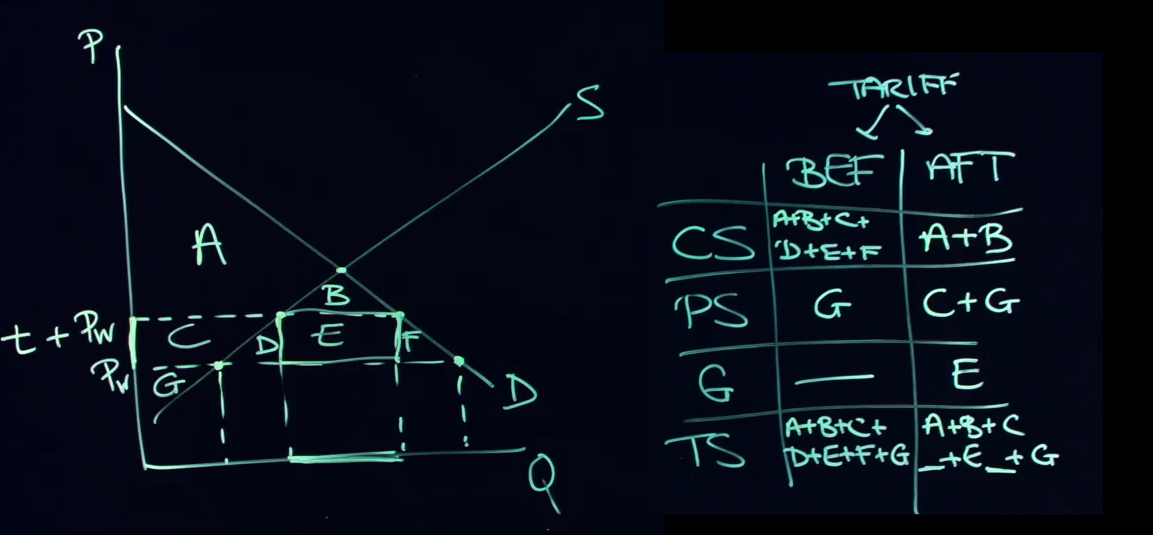
\includegraphics[width=0.5\textwidth]{Chapter20/Tariff.png}
    \caption{Tariff}
    \label{fig:tariff}
\end{figure}
D is the production distortion.\\
F is the consumption distortion.\\
Only the domestic producer surplus increases.\\
They get the government to put a tariff on the product.
\par
This story applies to small countries, what if a larger country pushes the tariff onto a smaller country?\\
This only works in limited circumstances.
\par
Instead of a price restriction (tariff) what if we had a quantity restriction (quota)?\\
The quota will be non-binding if the domestic demand is less than the imports.\\
The quota scenario is exactly the same as the tariff graph and table.\\
Quotas may lead to corruption.
\par
We can create a price discriminating monopoly (known as dumping). This is when a company sells a product at a lower price in a foreign country than in its home country.\\
The domestic consumer and foreign producer would be upset.\\
Foreign countries have the ability to retaliate by putting a tax (countervailing duty) on the product.